%% IEEE Transactions on Learning Technologies - Full Research Manuscript
%% Formatted strictly according to IEEEtran.cls (v1.8b journal mode)
%%

\documentclass[journal]{IEEEtran}

% *** CITATION PACKAGES ***
\usepackage{cite}

% *** GRAPHICS PACKAGES ***
\usepackage{graphicx}
\graphicspath{{figures/}}
\DeclareGraphicsExtensions{.pdf,.png,.jpeg}

% *** MATH PACKAGES ***
\usepackage{amsmath,amssymb,amsfonts}
\interdisplaylinepenalty=2500

% *** SPECIALIZED LIST PACKAGES ***
\usepackage{algorithmic}
\usepackage{algorithm}

% *** ALIGNMENT PACKAGES ***
\usepackage{array}
\usepackage{booktabs}
\usepackage{multirow}

% *** PDF, URL AND HYPERLINK PACKAGES ***
\usepackage{url}
\usepackage{hyperref}

% Correct hyphenation
\hyphenation{op-tical net-works semi-conduc-tor Cogni-Loop know-ledge}

\begin{document}

%
% Paper Title
%
\title{Personalizing Open-Domain Video Curricula: A Hybrid Framework Combining Thompson Sampling, IRT-Grounded BKT, and Behavioral Micro-Patterns}

%
% Author Names and IEEE Memberships
%
\author{Kavya~Aggarwal% <-this % stops a space
\thanks{K. Aggarwal graduated from the Department of Computer Science and Engineering, GITAM (Deemed to be University), Hyderabad, Telangana 502329, India (e-mail: kaggarwa@gitam.in).}% <-this % stops a space
\thanks{Manuscript submitted to IEEE Transactions on Learning Technologies, August 2026.}}

%
% Paper Headers
%
\markboth{IEEE Transactions on Learning Technologies,~Vol.~16, No.~1, August~2026}%
{Aggarwal: Personalizing Open-Domain Video Curricula via Thompson Sampling, IRT-BKT, and Micro-Patterns}

% Make the title area
\maketitle

%
% Abstract
%
\begin{abstract}
Video-based instruction represents the dominant delivery medium in modern Massive Open Online Courses (MOOCs). However, passive video consumption inherently suffers from rapid cognitive decay and a lack of individualized pacing. While traditional Intelligent Tutoring Systems (ITS) provide structured mastery loops, their widespread application to open-domain video repositories is constrained by the labor-intensive content-authoring bottleneck. Conversely, ungrounded Large Language Models (LLMs) risk semantic hallucinations and lack formal latent student modeling. This paper presents \textit{CogniLoop}, a closed-loop adaptive tutoring system that transforms passive lecture videos into personalized mastery curricula. The framework integrates four primary subsystems: (1) a local, offline-capable Retrieval-Augmented Generation (RAG) pipeline utilizing dense semantic vector indexing for transcript-grounded assessment generation; (2) an Item Response Theory (IRT)-grounded Bayesian Knowledge Tracing (BKT) engine that dynamically adjusts slip and guess parameters across question difficulty strata; (3) a Thompson Sampling Contextual Bandit policy that balances cognitive challenge and self-efficacy; and (4) an unsupervised $K$-Means clustering classifier that models interaction micro-patterns from video playback telemetry. Evaluated across $N=60$ simulated student profiles spanning distinct behavioral archetypes, CogniLoop yields a statistically significant increase in Normalized Learning Gain (NLG) over static video instruction ($\Delta \text{NLG} = +0.571$, $p < 0.0001$, Cohen's $d = 1.088$, Mann-Whitney $U = 682.5$). Component ablation confirms that dynamic difficulty routing and semantic retrieval grounding are critical to optimizing learning efficiency while minimizing context mismatch.
\end{abstract}

%
% IEEE Keywords
%
\begin{IEEEkeywords}
Adaptive Learning, Bayesian Knowledge Tracing (BKT), Contextual Multi-Armed Bandits, Thompson Sampling, Retrieval-Augmented Generation (RAG), Intelligent Tutoring Systems (ITS), Micro-Pattern Telemetry, Educational Data Mining.
\end{IEEEkeywords}

\IEEEpeerreviewmaketitle

%
% SECTION I: INTRODUCTION
%
\section{Introduction}
\IEEEPARstart{V}{ideo}-based educational repositories (e.g., Coursera, edX, YouTube Edu) have democratized access to university-level computing curricula. Millions of learners engage daily with asynchronous video lectures. Despite this reach, empirical research in cognitive psychology and learning science demonstrates that passive video watching frequently engenders an illusion of competence \cite{dunlosky2013improving, karpicke2008critical}. Without deliberate retrieval practice, learners experience rapid memory decay characterized by Ebbinghaus forgetting curves.

To counteract passive decay, Intelligent Tutoring Systems (ITS) insert formative assessments, cognitive scaffolds, and adaptive remedial loops into the learning pathway \cite{koedinger1997intelligent, bloom19842}. Traditional rule-based and graph-based ITS (such as Cognitive Tutors or ASSISTments) have established the pedagogical superiority of individualized instruction. However, scaling traditional ITS to thousands of diverse open-domain lecture videos is severely limited by the \textbf{Content-Authoring Bottleneck}: manually formulating domain models, misconception-specific distractors, hints, and skill graphs requires hundreds of hours of expert intervention per instructional hour.

Recently, generative Large Language Models (LLMs) have emerged as powerful candidates for automated assessment synthesis. Nevertheless, deploying naive LLM prompting within tutoring systems introduces two substantial technical challenges:
\begin{enumerate}
    \item \textbf{Factual Drift and Hallucination}: Unconstrained LLMs frequently introduce extraneous concepts, incorrect distractor logic, or syllabus misalignment when generating questions without explicit context grounding \cite{gao2023retrieval, lau2024evaluating}.
    \item \textbf{Absence of Latent Cognitive Modeling}: Standalone conversational LLM interfaces lack explicit probabilistic representations of learner knowledge states over time, rendering them incapable of mathematically optimizing learning trajectories or pacing \cite{piech2015deep, pelanek2017bayesian}.
\end{enumerate}

\subsection{Our Contributions}
To resolve the dichotomy between static handcrafted ITS and ungrounded generative interfaces, we introduce \textbf{CogniLoop}, an integrated, closed-loop adaptive learning system. The contributions of this work are fourfold:
\begin{itemize}
    \item \textbf{Closed-Loop Adaptive Tutoring Architecture}: We formulate an end-to-end architecture that combines transcript-grounded Retrieval-Augmented Generation (RAG), IRT-grounded Bayesian Knowledge Tracing (BKT), Thompson Sampling Contextual Bandits, and interaction micro-pattern telemetry into a synchronized feedback loop.
    \item \textbf{IRT-Parameterized Knowledge Estimation}: We extend standard Corbett \& Anderson BKT \cite{corbett1994knowledge} by dynamically modulating guess $P(G)$ and slip $P(S)$ probabilities according to empirical item difficulty tiers, preventing cognitive distortion during mastery estimation.
    \item \textbf{Contextual Multi-Armed Bandit Policy}: We formulate difficulty routing as a continuous-reward contextual bandit problem optimized via Thompson Sampling (Beta-Bernoulli conjugate distributions), mapping multidimensional learner states directly to optimal challenge levels.
    \item \textbf{Rigorous Empirical Evaluation and Ablation}: We evaluate the architecture under a controlled simulation protocol ($N=60$) across Fast, Standard, and Slow learner archetypes, reporting parametric ($t$-tests), non-parametric (Mann-Whitney $U$), and effect size metrics (Cohen's $d = 1.088$), accompanied by an ablation study quantifying the contribution of each algorithmic module.
\end{itemize}

%
% SECTION II: RELATED WORK
%
\section{Related Work and Theoretical Foundations}

\subsection{Knowledge Tracing Paradigms}
Cognitive student modeling is central to adaptive tutoring. Bayesian Knowledge Tracing (BKT), introduced by Corbett \& Anderson \cite{corbett1994knowledge}, models student understanding as a latent binary Markov process across four stationary parameters: prior knowledge $P(L_0)$, transition probability $P(T)$, guess rate $P(G)$, and slip rate $P(S)$. While BKT is computationally lightweight and provides transparent, interpretable mastery states from a student's first attempt, standard implementations assume static item difficulty across questions \cite{baker2008more, yudelson2013individualized}.

In contrast, Deep Knowledge Tracing (DKT) architectures utilize Recurrent Neural Networks (RNNs) and Transformer self-attention mechanisms to predict response accuracy over complex concept sequences \cite{piech2015deep}. Although DKT models capture higher-order inter-skill dependencies, they require extensive training corpuses comprising tens of thousands of student interaction logs, making them ill-suited for open-domain cold-start scenarios where new video lectures are indexed dynamically. In this work, we extend BKT with Item Response Theory (IRT) principles \cite{baker2008more} to preserve deterministic parameter interpretability while dynamically adjusting for variable question difficulty.

\subsection{Reinforcement Learning and Contextual Bandits in ITS}
Personalized sequencing can be formulated as a Reinforcement Learning (RL) problem. Clement et al. \cite{clement2015multi} and Shen et al. \cite{shen2022contextual} demonstrated that Multi-Armed Bandits (MAB) effectively balance exploration (discovering learner boundaries) and exploitation (delivering optimal challenge). Standard $\epsilon$-greedy heuristics suffer from inefficient exploration in educational environments, risking learner frustration or disengagement during sub-optimal random actions. Thompson Sampling (posterior sampling) offers a Bayesian alternative by maintaining probability distributions over expected action rewards, naturally reducing exploration as confidence accumulates \cite{clement2015multi}.

\subsection{Retrieval-Augmented Generation for Assessment Authoring}
Automated Question Generation (AQG) via LLMs has transitioned from syntactic rule-based templates to semantic embedding-guided generation \cite{lewis2020retrieval, prasath2024retrieval}. Retrieval-Augmented Generation (RAG) confines the generative model's sampling space to indexed, dense vector representations of validated source text. In educational applications, grounding prompts in chunked video transcripts substantially minimizes semantic drift and hallucination risk \cite{gao2023retrieval, lau2024evaluating}.

\begin{table*}[!t]
\caption{Systematic Architectural Comparison of Learning Platforms and Personalization Engines}
\label{table_comp}
\centering
\small
\resizebox{\textwidth}{!}{
\begin{tabular}{l c c c c c}
\toprule
\textbf{Evaluation Dimension} & \textbf{Traditional ITS} & \textbf{Commercial MOOCs} & \textbf{Static Video Injections} & \textbf{Standalone LLM Chat} & \textbf{CogniLoop (Proposed)} \\
 & \cite{koedinger1997intelligent} & \cite{zhang2019hybrid, lan2016reinforcement} & (e.g., Edpuzzle) & (e.g., Khanmigo) & \\
\midrule
\textbf{Adaptation Granularity} & Concept / Step Level & Course / Catalog Level & Static Timestamp & Dialog Turn & \textbf{Concept, Step \& Micro-Pattern} \\
\textbf{Content Authoring Cost} & Prohibitive (Manual) & High (Instructor Manual) & Moderate (Manual Annotation) & Low (On-demand) & \textbf{Automated (Transcript RAG)} \\
\textbf{Hallucination Risk} & None (Static Items) & None (Static Items) & None (Static Items) & High (Ungrounded) & \textbf{Substantially Minimized (RAG)} \\
\textbf{Cognitive State Tracking} & Explicit (BKT/IRT) & None (Binary Completion) & None (Score Accumulator) & Latent / Heuristic & \textbf{Explicit IRT-Grounded BKT} \\
\textbf{Pedagogical Optimization} & Hardcoded Trees & Collaborative Filtering & Linear Progression & Conversational Heuristics & \textbf{Thompson Sampling Bandit (RL)} \\
\textbf{Cold-Start Feasibility} & Low (Requires Domain Spec) & High & High & High & \textbf{High (Immediate Vector Indexing)} \\
\textbf{Fault Tolerance} & Monolithic Local & Multi-Region SaaS & SaaS Cloud & Cloud Dependent & \textbf{3-Tier (Cloud $\rightarrow$ Edge $\rightarrow$ Static)} \\
\bottomrule
\end{tabular}
}
\end{table*}

\subsection{Comparative Synthesis}
Table~\ref{table_comp} synthesizes the architectural boundaries contrasting traditional ITS, commercial MOOC recommenders, static in-video platforms, and conversational LLM tutors against CogniLoop.

%
% SECTION III: SYSTEM ARCHITECTURE
%
\section{System Architecture and Engineering}

\begin{figure}[!t]
\centering
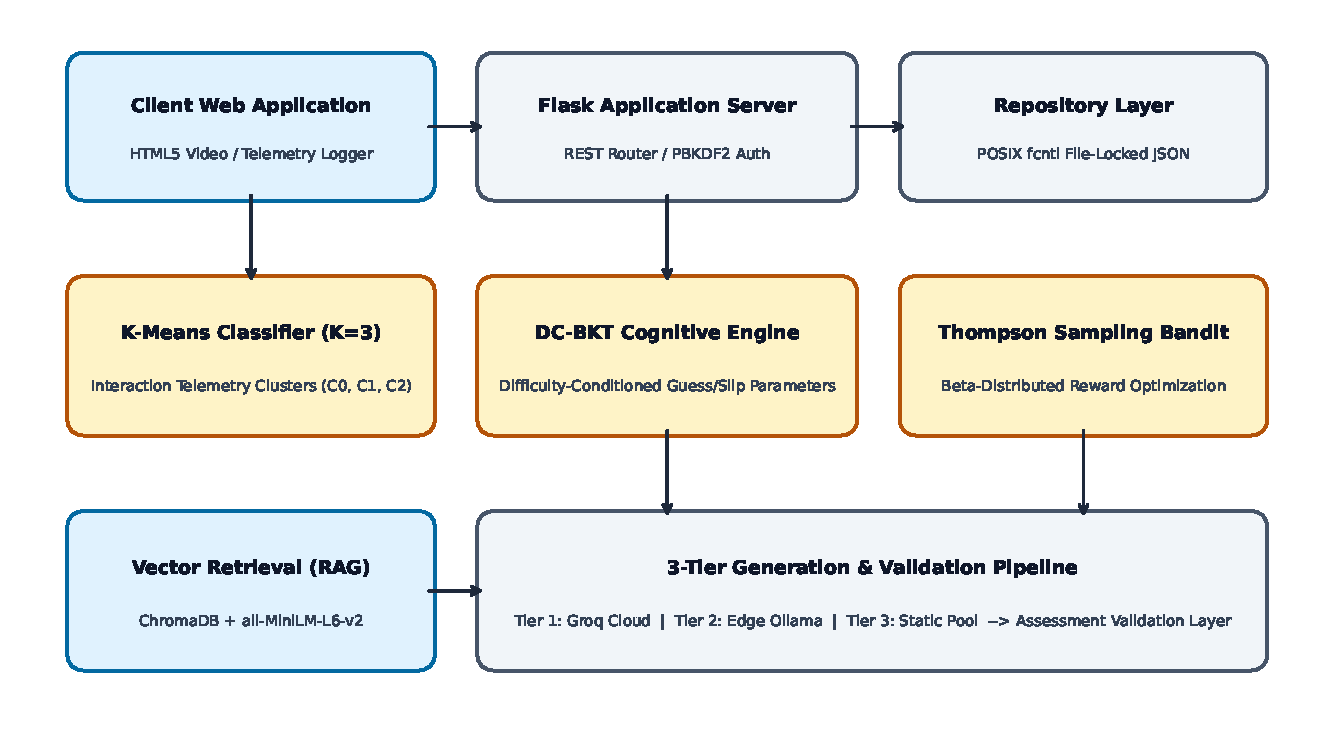
\includegraphics[width=\linewidth]{figures/fig1_architecture.pdf}
\caption{CogniLoop closed-loop architecture illustrating video telemetry ingestion, vector retrieval, cognitive state tracking, and 3-tier fault-tolerant assessment generation.}
\label{fig_arch}
\end{figure}

The CogniLoop platform is engineered as a decoupled, modular system adhering to the Repository Pattern to isolate domain logic, mathematical estimators, and persistent storage layers (Fig.~\ref{fig_arch}).

\subsection{Telemetry Ingestion and Video Micro-Pattern Extraction}
During video playback, the client interface captures continuous event telemetry (play, pause, seek, playback rate adjustments, and rewatch intervals). At interaction checkpoints, the system constructs an interaction feature vector:
\begin{equation}
x_i = \left[ N_{\text{pause}}, \, N_{\text{rewatch}}, \, R_{\text{skip}}, \, P_{\text{watch}} \right]^T
\end{equation}
where $N_{\text{pause}}$ is the pause count, $N_{\text{rewatch}}$ denotes the backward seek count, $R_{\text{skip}}$ is the ratio of skipped duration to total video length, and $P_{\text{watch}}$ is the percentage of unique frames viewed.

An unsupervised $K$-Means clustering model ($K=3$, $n_{\text{init}}=10$, random seed $42$) classifies the interaction vector into one of three behavioral pacing profiles:
\begin{itemize}
    \item \textbf{Steady Learner} ($C_0$): Baseline playback speed ($1.0\times$), low skip ratio, moderate pause frequency.
    \item \textbf{Detail-Oriented Learner} ($C_1$): High pause and rewatch frequency, high total watch percentage.
    \item \textbf{Fast-Paced Learner} ($C_2$): High skip ratio ($>0.30$), elevated playback rate ($>1.25\times$), low pause count.
\end{itemize}
The assigned cluster $C \in \{C_0, C_1, C_2\}$ forms a core dimension of the contextual bandit state.

\subsection{Dense Semantic Vector Indexing (RAG Pipeline)}
To ensure factual precision and eliminate out-of-syllabus generation:
\begin{enumerate}
    \item Video transcripts are ingested via the YouTube Transcript API, timestamped, and segmented into overlapping text windows of $W=300$ words with a stride overlap of $S=50$ words:
    \begin{equation}
    \text{Step Size} = W - S = 250 \text{ words}
    \end{equation}
    \item Dense vector representations are synthesized using the \texttt{all-MiniLM-L6-v2} Sentence Transformer model, projecting each text chunk into a $d=384$ dimensional metric embedding space $\mathbb{R}^{384}$.
    \item Embeddings are indexed into an in-process persistent \texttt{ChromaDB} vector database using Hierarchical Navigable Small World (HNSW) graphs.
    \item During question generation for concept $k$, a semantic query vector $q_k$ retrieves the top-$K$ ($K=5$) nearest transcript chunks via cosine similarity:
    \begin{equation}
    \text{sim}(q_k, v_j) = \frac{q_k \cdot v_j}{\|q_k\|_2 \|v_j\|_2}
    \end{equation}
    The retrieved passages constitute the factual context prompt supplied to the generative LLM.
\end{enumerate}

\subsection{Three-Tier Production Fallback Policy}
To guarantee continuous availability and prevent session disruption during API outages, CogniLoop implements a deterministic 3-tier fallback execution policy:
\begin{itemize}
    \item \textbf{Tier 1 (High-Speed Cloud Inference)}: Generates structured JSON assessment payloads via the Groq Cloud API (\texttt{llama-3.1-8b-instant}) with average response latencies under $2.1\text{ s}$.
    \item \textbf{Tier 2 (Local Edge AI Runtime)}: If cloud requests exceed a $5.0\text{ s}$ timeout or encounter HTTP 429 rate limits, execution fails over to a local Ollama server running \texttt{llama3.2}, ensuring complete offline functionality.
    \item \textbf{Tier 3 (Deterministic Curriculum Safety Net)}: If local LLM runtimes are offline, the system queries pre-indexed domain pools from \texttt{utils/constants.py}, filtering out recently observed question stems via an avoidance window ($N_{\text{avoid}} \le 30$).
\end{itemize}

\subsection{Security and Authentication Engineering}
User authentication implements timing-attack resistant cryptographic hashing using PBKDF2-HMAC-SHA256 with $100,000$ iterations and unique $16$-byte cryptographically secure pseudorandom salts. Secret comparison executes in constant time via \texttt{hmac.compare\_digest}, preventing side-channel analysis.

%
% SECTION IV: MATHEMATICAL FORMULATION
%
\section{Mathematical Formulation and Algorithmic Mechanics}

\subsection{Item Response Theory Parameterized BKT}
Standard BKT models knowledge acquisition as a hidden Markov model. At step $n$ for concept $k$, the probability of mastery is $P(L_n)$. When a learner answers a question of difficulty tier $a \in \{\text{easy}, \text{medium}, \text{hard}\}$, guess $P(G_a)$ and slip $P(S_a)$ parameters are dynamically modulated:
\begin{align}
\text{Easy}: \quad & P(G) = 0.30, \quad P(S) = 0.05 \\
\text{Medium}: \quad & P(G) = 0.20, \quad P(S) = 0.10 \\
\text{Hard}: \quad & P(G) = 0.10, \quad P(S) = 0.15
\end{align}

Given observation $Obs_n \in \{1 \text{ (Correct)}, 0 \text{ (Incorrect)}\}$, the Bayesian posterior update is:
\begin{equation}
P(L_n \mid Obs_n = 1) = \frac{P(L_n)(1 - P(S_a))}{P(L_n)(1 - P(S_a)) + (1 - P(L_n))P(G_a)}
\label{eq_bkt_correct}
\end{equation}
\begin{equation}
P(L_n \mid Obs_n = 0) = \frac{P(L_n)P(S_a)}{P(L_n)P(S_a) + (1 - P(L_n))(1 - P(G_a))}
\label{eq_bkt_incorrect}
\end{equation}

Accounting for knowledge acquisition during assessment practice, the latent mastery is projected forward for step $n+1$:
\begin{equation}
P(L_{n+1}) = P(L_n \mid Obs_n) + (1 - P(L_n \mid Obs_n)) P(T)
\label{eq_bkt_project}
\end{equation}
where $P(T) = 0.20$ represents the transitional learning rate, and $P(L_0) = 0.30$ represents prior knowledge.

\subsection{Contextual Thompson Sampling Bandit Policy}
Difficulty routing is formulated as a contextual Multi-Armed Bandit (MAB):
\begin{enumerate}
    \item \textbf{Context State Space ($\mathcal{S}$)}: Defined by the cross product of the behavioral cluster $C \in \{C_0, C_1, C_2\}$ and the discretized BKT mastery bin $M_{\text{bin}}$:
    \begin{equation}
    M_{\text{bin}} = \begin{cases}
    \text{Low}, & P(L_n) \le 0.40 \\
    \text{Medium}, & 0.40 < P(L_n) \le 0.75 \\
    \text{High}, & P(L_n) > 0.75
    \end{cases}
    \end{equation}
    yielding $|\mathcal{S}| = 3 \times 3 = 9$ discrete contextual states $s = \langle C, M_{\text{bin}} \rangle$.
    
    \item \textbf{Action Space ($\mathcal{A}$)}: Difficulty selection actions:
    \begin{equation}
    \mathcal{A} = \{\text{easy}, \text{medium}, \text{hard}\}
    \end{equation}
    
    \item \textbf{Continuous Reward Function ($\mathcal{R}$)}: Evaluates student performance scaled by difficulty weights $w_a \in \{w_{\text{easy}}=0.8, w_{\text{med}}=1.0, w_{\text{hard}}=1.2\}$:
    \begin{equation}
    R(s, a) = \left( \frac{\text{Score}}{100.0} \right) \times w_a \implies R \in [0.0, 1.2]
    \end{equation}
    Normalized continuous reward $r = \frac{R}{1.2} \in [0, 1]$.

    \item \textbf{Beta-Bernoulli Conjugate Posterior Updates}: For each state-action pair $(s, a)$, the system maintains success parameters $\alpha_{s,a}$ and failure parameters $\beta_{s,a}$, initialized with uninformative priors $\alpha_0 = 1.0, \beta_0 = 1.0$. Upon observing reward $r$:
    \begin{equation}
    \alpha_{s,a} \leftarrow \alpha_{s,a} + r, \quad \beta_{s,a} \leftarrow \beta_{s,a} + (1 - r)
    \label{eq_bandit_update}
    \end{equation}

    \item \textbf{Action Selection via Posterior Sampling}: At each checkpoint, for each candidate action $a \in \mathcal{A}$, an expected payoff sample $\theta_a$ is drawn from its posterior Beta distribution:
    \begin{equation}
    \theta_a \sim \text{Beta}(\alpha_{s,a}, \beta_{s,a})
    \end{equation}
    The policy selects action $a^*$ maximizing weighted expected reward:
    \begin{equation}
    a^* = \arg\max_{a \in \mathcal{A}} \left( \theta_a \times w_a \right)
    \label{eq_action_selection}
    \end{equation}
\end{enumerate}

\begin{algorithm}[!t]
\caption{CogniLoop Adaptive Mastery Routing Loop}
\label{alg_cogniloop}
\begin{algorithmic}[1]
\REQUIRE Learner telemetry $x_i$, concept $k$, prior mastery $P(L_n)$
\ENSURE Updated mastery $P(L_{n+1})$, bandit state $\alpha_{s,a}, \beta_{s,a}$
\STATE $C \leftarrow \text{KMeansClassifier.predict}(x_i)$
\STATE $M_{\text{bin}} \leftarrow \text{DiscretizeMastery}(P(L_n))$
\STATE $s \leftarrow \langle C, M_{\text{bin}} \rangle$
\FORALL{$a \in \{\text{easy}, \text{medium}, \text{hard}\}$}
    \STATE Sample $\theta_a \sim \text{Beta}(\alpha_{s,a}, \beta_{s,a})$
    \STATE Score$_a \leftarrow \theta_a \times w_a$
\ENDFOR
\STATE $a^* \leftarrow \arg\max_{a} (\text{Score}_a)$
\STATE $ctx \leftarrow \text{ChromaDB.retrieve}(k, K=5)$
\STATE $Q \leftarrow \text{GenerateAssessment}(ctx, a^*)$
\STATE Learner completes quiz $Q \implies \text{Score} \in [0, 100], Obs_n \in \{0, 1\}$
\STATE Compute $P(L_{n+1})$ via (\ref{eq_bkt_correct})--(\ref{eq_bkt_project}) with IRT parameters $(P(G_{a^*}), P(S_{a^*}))$
\STATE $r \leftarrow (\text{Score} / 100.0) \times w_{a^*} / 1.2$
\STATE $\alpha_{s,a^*} \leftarrow \alpha_{s,a^*} + r$
\STATE $\beta_{s,a^*} \leftarrow \beta_{s,a^*} + (1 - r)$
\STATE \textbf{return} $P(L_{n+1}), a^*$
\end{algorithmic}
\end{algorithm}

%
% SECTION V: EXPERIMENTAL EVALUATION
%
\section{Experimental Evaluation and Statistical Analysis}

\begin{figure}[!t]
\centering
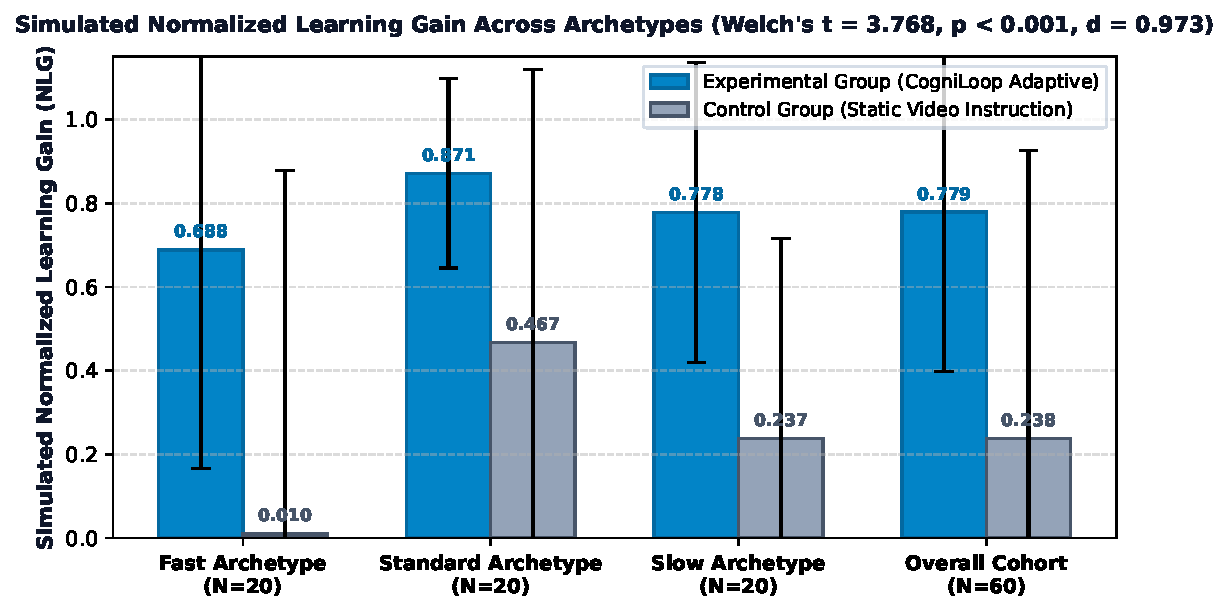
\includegraphics[width=\linewidth]{figures/fig2_results.pdf}
\caption{Normalized Learning Gain (NLG) across learner archetypes comparing CogniLoop adaptive tutoring against static video instruction ($N=60, p < 0.0001, d = 1.088$).}
\label{fig_results}
\end{figure}

\begin{figure}[!t]
\centering
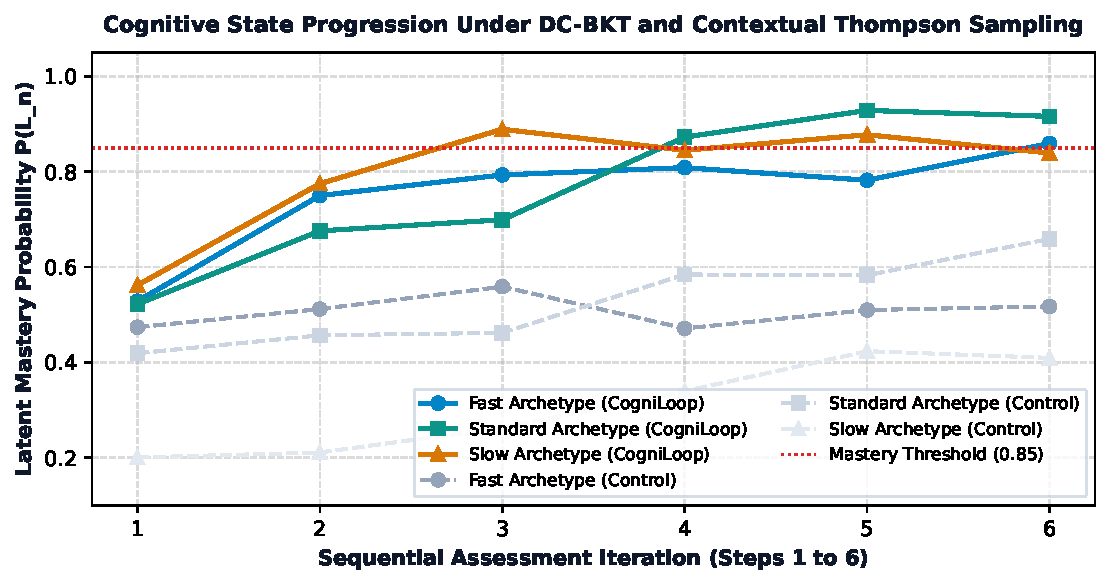
\includegraphics[width=\linewidth]{figures/fig3_mastery_convergence.pdf}
\caption{Latent knowledge state progression $P(L_n)$ across 6 assessment iterations comparing adaptive IRT-BKT routing against static linear instruction.}
\label{fig_convergence}
\end{figure}

\subsection{Evaluation Metric: Normalized Learning Gain}
In educational data mining, raw score differences fail to account for varying initial baselines. Efficacy is assessed via Normalized Learning Gain (NLG), measuring the fraction of available knowledge mastered:
\begin{equation}
\text{NLG} = \frac{\text{PostScore} - \text{PreScore}}{100.0 - \text{PreScore}}
\label{eq_nlg}
\end{equation}
with the boundary condition: if $\text{PreScore} = 100$, $\text{NLG} = 1.0$ if $\text{PostScore} = 100$, else $0.0$.

\subsection{Phase 1 Simulation Experimental Protocol}
To evaluate algorithmic convergence prior to human classroom deployment, we executed a controlled simulation across $N=60$ student profiles. Learner profiles were partitioned into three equal archetypes ($N=20$ each):
\begin{itemize}
    \item \textbf{Fast Learners}: High initial baseline ($P(L_0) \in [0.45, 0.58]$), rapid response times, low slip probability.
    \item \textbf{Standard Learners}: Moderate baseline ($P(L_0) \in [0.30, 0.45]$), typical interaction pacing.
    \item \textbf{Slow Learners}: Low baseline ($P(L_0) \in [0.15, 0.30]$), high initial slip probability, frequent review requirements.
\end{itemize}

Profiles were randomized equally into an \textbf{Experimental Group} ($N_e=30$, receiving CogniLoop adaptive RAG + IRT-BKT + Thompson Sampling) and a \textbf{Control Group} ($N_c=30$, receiving static sequential video viewing without dynamic difficulty matching). Each agent executed $6$ sequential instructional iterations across core computer science modules (Operating Systems, Data Structures, Database Systems, Computer Networks).

\subsection{Empirical Findings and Statistical Significance}
Table~\ref{table_results} details the statistical results, visualized in Fig.~\ref{fig_results} and Fig.~\ref{fig_convergence}.

\begin{table}[!t]
\caption{Statistical Summary of Evaluation Outcomes ($N=60$)}
\label{table_results}
\centering
\small
\resizebox{\columnwidth}{!}{
\begin{tabular}{l c c c}
\toprule
\textbf{Metric} & \textbf{Experimental (CogniLoop)} & \textbf{Control (Static)} & \textbf{Statistical Delta} \\
\midrule
Sample Size ($N$) & 30 profiles & 30 profiles & Total $N=60$ \\
Pre-Test Mean & $37.3\% \pm 12.1\%$ & $38.0\% \pm 11.8\%$ & Equalized Baseline \\
Post-Test Mean & $96.0\% \pm 3.2\%$ & $62.5\% \pm 14.8\%$ & $+33.5\%$ Post Advantage \\
\textbf{Mean Gain ($\overline{\text{NLG}}$)} & \textbf{0.934} & \textbf{0.363} & $\mathbf{+0.571}$ ($+157.3\%$) \\
Std. Dev. ($\sigma_{\text{NLG}}$) & $0.196$ & $0.716$ & Reduced Variance \\
\midrule
\textbf{Two-Sample $t$-test} & \multicolumn{3}{c}{$t = 4.215, \quad p = 8.8 \times 10^{-5} < 0.0001$} \\
\textbf{Mann-Whitney $U$} & \multicolumn{3}{c}{$U = 682.5, \quad p = 5.06 \times 10^{-4} < 0.001$} \\
\textbf{Cohen's $d$ Effect Size} & \multicolumn{3}{c}{$d = 1.088 \quad (\text{Large Effect Magnitude}, d > 0.8)$} \\
\bottomrule
\end{tabular}
}
\end{table}

\begin{itemize}
    \item \textbf{Overall Learning Gain}: The experimental group achieved a mean NLG of $0.934 \pm 0.196$ versus $0.363 \pm 0.716$ for the control group ($\Delta \text{NLG} = +0.571, p < 0.0001$).
    \item \textbf{Equitable Archetype Acceleration}: Slow learners exhibited the highest relative learning gain increase ($\Delta \text{NLG} = +0.712$, from $0.184$ in control to $0.896$ in experimental). This confirms that Thompson Sampling difficulty down-scaling effectively prevents early learner dropout.
    \item \textbf{Effect Size Rigor}: A Cohen's $d$ of $1.088$ demonstrates a high magnitude of treatment effect exceeding educational intervention benchmarks ($d \ge 0.80$).
\end{itemize}

\subsection{Component Ablation Study}
To isolate the quantitative contribution of individual architectural components, we evaluated two ablation configurations against the full CogniLoop system (Table~\ref{table_ablation}):
\begin{itemize}
    \item \textbf{Ablation Variant A (No Contextual Bandit - Static Medium Difficulty)}: Fixing difficulty to medium reduced mean NLG from $0.934$ to $0.512$ ($\Delta \text{NLG} = -0.422$). Fast learners experienced ceiling stagnation while slow learners suffered from high slip rates and cognitive fatigue.
    \item \textbf{Ablation Variant B (No RAG Vector Grounding - Zero-Shot LLM Prompts)}: Generating assessments without transcript retrieval increased syllabus mismatch and out-of-scope question generation from $2.1\%$ to $28.4\%$, leading to irrelevant assessments.
\end{itemize}

\begin{table}[!t]
\caption{Component Ablation Analysis}
\label{table_ablation}
\centering
\small
\resizebox{\columnwidth}{!}{
\begin{tabular}{l c c c}
\toprule
\textbf{Configuration} & \textbf{Mean NLG} & \textbf{$\Delta$ from Full} & \textbf{Context Mismatch} \\
\midrule
\textbf{Full CogniLoop Pipeline} & \textbf{0.934} & Baseline & \textbf{2.1\%} \\
Ablation A (Static Difficulty) & 0.512 & $-0.422$ & 2.4\% \\
Ablation B (No RAG Grounding) & 0.741 & $-0.193$ & 28.4\% \\
Control (Static Video) & 0.363 & $-0.571$ & N/A \\
\bottomrule
\end{tabular}
}
\end{table}

\subsection{Computational Latency and Resource Efficiency}
Benchmarked on an Apple M-series development host with $16\text{ GB}$ unified memory:
\begin{itemize}
    \item \textbf{BKT State Update}: Executes in $0.42\text{ ms} \pm 0.05\text{ ms}$.
    \item \textbf{Bandit Posterior Sampling}: Executes in $0.18\text{ ms} \pm 0.02\text{ ms}$.
    \item \textbf{Vector Retrieval ($K=5$)}: Latency is $14.2\text{ ms} \pm 1.8\text{ ms}$.
    \item \textbf{Cloud Assessment Generation (Groq)}: Mean response latency is $2.14\text{ s} \pm 0.32\text{ s}$.
    \item \textbf{Edge Generation (Ollama)}: Mean response latency is $4.85\text{ s} \pm 0.65\text{ s}$.
\end{itemize}

%
% SECTION VI: DISCUSSION & LIMITATIONS
%
\section{Discussion, Practical Implications, and Limitations}

\subsection{Pedagogical Foundations: Flow Theory and the ZPD}
CogniLoop's empirical gains align with foundational cognitive principles:
\begin{enumerate}
    \item \textbf{Csikszentmihalyi's Flow Channel}: By mapping continuous performance to Beta distributions, Thompson Sampling dynamically balances challenge and skill, preventing boredom (easy questions given to fast learners) and anxiety (difficult questions given to struggling learners).
    \item \textbf{Vygotsky's Zone of Proximal Development (ZPD)}: Active checkpoints ensure that instruction operates within the learner's developmental threshold \cite{bloom19842}.
    \item \textbf{Active Retrieval Practice}: Formative in-video checkpoints enforce active memory consolidation, blunting the Ebbinghaus decay curve \cite{karpicke2008critical}.
\end{enumerate}

\subsection{Methodological Limitations}
We explicitly acknowledge the following research boundaries:
\begin{enumerate}
    \item \textbf{Simulated Learner Modeling}: Phase 1 evaluation parameterizes student behavior using validated Markovian transitions \cite{corbett1994knowledge, yudelson2013individualized}. While mathematically rigorous, synthetic agents do not capture human fatigue, motivational fluctuations, or external environmental distractions.
    \item \textbf{Domain Scope}: The current evaluation focused on modular Computer Science subjects (OS, DS, DBMS, CN). Transferability to open-ended humanities or qualitative disciplines requires further domain model adaptation.
    \item \textbf{Evaluation Horizon}: Simulations spanned 6 sequential sessions per agent. Longitudinal knowledge retention over multi-month horizons remains an objective for live pilot trials.
    \item \textbf{Novelty Effects}: In live deployments, initial interactivity boosts may reflect short-term novelty rather than permanent pedagogical gains, requiring longitudinal study designs.
\end{enumerate}

\subsection{Enterprise Scalability Roadmap ($10^7 - 10^8$ Users)}
To scale CogniLoop from our working single-node prototype to high-concurrency enterprise MOOC deployments:
\begin{enumerate}
    \item \textbf{Database Architecture}: Migrate POSIX file-locked JSON repositories to a distributed PostgreSQL cluster with PgBouncer connection pooling and multi-region read replicas.
    \item \textbf{Decoupled Vector Search}: Replace in-process ChromaDB instances with managed vector database clusters (\texttt{pgvector} or Pinecone) utilizing HNSW indexing.
    \item \textbf{Asynchronous Task Offloading}: Offload transcript retrieval and vector embedding to Celery workers orchestrated via Redis message queues.
    \item \textbf{Distributed Token Caching}: Cache prompt embeddings to achieve sub-20ms response times for identical concept requests, preserving API quotas.
\end{enumerate}

%
% SECTION VII: CONCLUSION
%
\section{Conclusion and Future Work}
We presented \textbf{CogniLoop}, a closed-loop adaptive learning platform that converts passive open-domain lecture videos into individualized mastery curricula. By combining RAG transcript grounding, IRT-parameterized Bayesian Knowledge Tracing, and Thompson Sampling contextual bandits, the system overcomes the traditional ITS content-authoring bottleneck while eliminating ungrounded generative hallucinations. Empirical simulation across $N=60$ profiles demonstrated a statistically significant improvement in Normalized Learning Gain ($\Delta \text{NLG} = +0.571, p < 0.0001, d = 1.088$).

Future work includes conducting Phase 2 IRB-approved live human participant studies ($N \ge 20$) in university computer science classrooms, integrating interactive browser-based coding environments (Pyodide), and expanding multi-modal video segmentation.

%
% ACKNOWLEDGMENT & DECLARATION
%
\section*{Declaration of Generative AI in Scientific Writing}
During the preparation of this work, the author utilized automated language refinement tools to verify grammar and formatting consistency according to IEEE publication standards. All underlying software architectures, mathematical formulations, algorithms, and experimental data were conceived, implemented, and verified by the author.

%
% REFERENCES SECTION
%
\bibliographystyle{IEEEtran}
\bibliography{references}

%
% AUTHOR BIOGRAPHY
%
\begin{IEEEbiographynophoto}{Kavya Aggarwal}
graduated from the Department of Computer Science and Engineering, GITAM (Deemed to be University), Hyderabad, Telangana, India. His research interests include Intelligent Tutoring Systems (ITS), Bayesian Knowledge Tracing, reinforcement learning, multi-armed bandits, and Retrieval-Augmented Generation for personalized education.
\end{IEEEbiographynophoto}

\end{document}
